\chapter{Design Outline}\label{design outline}\label{section \thechapter}

\mySection{Aims and motivations}{\AG}\label{outline aims and motivations}
\todo{This section is identical to Section~\ref{summary: why}. Here should be some options for motivations and reasons for them, perhaps? (More in keeping with the rest of the chapter.)}
The invention of the difference engine in 1833, came with it an entire new process of thought and development. Since then, the field of computation and robotics has become one of the largest in the world. It is a field that requires developers to suspend their usual way of thinking and instead look at tasks and problems as a computer. These ways of thinking are not encountered in daily life. Other intellectual and physical fields have their foundations discovered through juvenile interactions. However, the ability to approach a task with an algorithmic method---a loop or conditional statements---is not naturally acquired. These skills must therefore be taught through non-conventional means. This could be as a teenager or adult, when first being confronted with programming; however, years of educational studies have shown that skills and understanding are much more easily acquired at an early age. This is the motivation of the \SandE project: to develop a method, useable by schools and parents, to begin to nurture programming skills in children.

The aim for this project is to develop a working prototype of a programmable, autonomous robot with the ability to draw large scale art in sand. The robot will be able to accept a set of repeatable instructions from a student. These instructions could include: navigation, for example an instruction to go from point A to B before turning and traveling to point C; the ability to control whether the robot should be drawing at any given time, and also the thickness of the line drawn. The student will create these instructions through a graphical user interface, before they are uploaded to the robot and their design is created in sand. The intention is that by passing a design to a robot, students will be forced to think about how a computer will tackle a task they would find simple. Hopefully, students will be able to understand that computers use a system of specific logic that can create wonderful things, which would take much longer by hand.


\mySection{Movement}{\SW}
    In considering the robot's locomotion, the terrain over which it will travel (sand -- potentially damp) and its purpose (drawing) are center-stage. The robot must have sufficient traction to travel over a beach. When considering the requirement that it draw, it must be able to turn as tightly as instructed to avoid incongruity between programmed and drawn images. It may also be possible to incorporate any turning limitations into the child's programming interface, such that an impossible turn cannot be instructed. It would also be far from ideal for the robot to obscure any lines it had already drawn when pathing back over them.

    The main methods of robot locomotion that might be relevant are wheeled (or caterpillar tracked), walking, rolling, or slithering. Considering the scope of this project, and the budget available, the latter options are not viable. Companies such as Boston Dynamics have budgets of millions of dollars to work on the development of walking technology -- achieving a robot capable of walking is a significant feat, even before considering drawing. While rolling or slithering may potentially be workable, they would contribute significant design complications to any kind of `on/off' functionality. Flying private drones have increased in popularity dramatically; in considering a drone type robot as an option, the main challenges are the extreme comparative difficulty of achieving flight compared with traction and drawing a line in the sand. Creating a flying drone from scratch would pose many challenges, which it is unlikely we could surmount with this project's resources. The marker design also poses significant challenges -- a marker fixed rigidly to a drone is likely to interfere with flight and a free-hanging marker runs the risk of not providing enough pressure to create a line. The most viable locomotion solutions are caterpillar tracks and wheels.\\
    Caterpillar tracks combine very capable terrain handling with on-a-point turning, however they are very likely to disrupt the line left behind the robot, especially when on-a-point turning.  With the right design and material, wheels might prove sufficiently able to handle the terrain and also cause limited harm to the robot's drawn lines. Such wheels would need to have a large surface area and be made of a reasonably soft material (\eg soft touch plastic) -- minimizing the robot's overall weight would also be important in making such a design choice viable. Although wheels open opportunities in terrain handling and line preservation, they come up short of caterpillar tracks on turning ability. A short wheelbase might go some way to improve this. There is also the potential of a three-wheel configuration, instead of four (or more) wheels -- this was implemented in Disney's BeachBot (Section~\ref{sand-drawing robots}) to the benefit of the robot’s turning circle. It should be noted that a three-wheel design raises stability concerns. Ultimately the decision between caterpillar tracks and wheels comes to a question of whether, or to what extent, the child instructing the robot should be limited in their design.

\mySection{Digging mechanism}{\SW}
    At its most basic level, a beach-scale sand drawing robot need only leave a line in the sand wherever it travels, in order to produce a picture -- this poses a severe constraint on what can be drawn. In the case of our educational robot, the child would have the limitation of instructing the robot to draw a picture with only a single continuous movement. This `always on' approach to the drawing mechanism can be improved upon.

    Instead of fixing the robot's marking implement, it could be built to raise or lower, adding `on/off' drawing functionality. The marking implement, or `marker', could be fitted to an actuator to achieve this. The actuator could be linear or rotary; a linear actuator would lend itself to a marker below the robot chassis, while a rotary actuator would be more appropriate for a marker behind the chassis, like a rake tooth (as is being used in Figure~\ref{fig: andres amador}). A rear mounted, rake-like design might provide a more fluid, pulling movement through the sand. There are precedents for this positioning choice: Disney's BeachBot (Section~\ref{sand-drawing robots}) and plough attachments for tractors. While the addition of an actuator significantly improves the robot's drawing flexibility, it would be vulnerable to sand in its mechanism and would add cost, should one not be salvageable from spare parts. The use of an actuator would also place a small requirement on the robot's power supply.\\
    The marker itself needs to exert sufficient force on the sand to leave a line behind the robot, without acting as a brake -- this would inhibit the robot's movement. Inhibition of the robot's movement would lead to significant deviation in the drawn image compared to the programmed image. The key to avoiding this is to create a marker with appropriate depth; the marker should not penetrate so deep in the sand as to invite significant resistance to its motion, while reaching deep enough to leave a sufficient (\emph{i.e.} visible) line.\\
    Implementing software to vary the depth of the marker could serve to mitigate any issues arising from resistance, and also could ensure trouble does not arise on uneven beach area. The limitations here lie within the realm of software development, and potentially the requirement that the actuator provide feedback.\\
    Within these parameters the marker itself could be varied -- for instance having multiple markers would provide a different pattern to the line. These multiple markers could be fitted to more actuators (with the potential of substantially increased cost) to allow for a variable line width.

    An alternative marker approach would be that of a cylindrical `drum'. Such a cylinder could have a pattern embossed upon it that would leave a pattern as the robot's marking. Gunilla Klingberg's `sand machine' (Section~\ref{art review}, Figure~\ref{fig: sand machine}) uses this approach. This approach could be implemented with `on/off' functionality, but would allow for only a preset pattern in the line. The implementation of a patterned line of varying width (\eg multiple drums with raising and lowering ability) could prove very problematic. Such an implementation of this method would be best achieved in a manner similar to NASA's RASSOR digging robot -- a drum separate from the locomotion mechanism that can be lowered and raised.\cite{Siceloff2013} In a similar way, the NASA's Curiosity rover leaves the pattern for ``JPL'' in Morse code in its tracks as it travels across the Martian surface.


\mySection{Interface}{writer TBA}
\towrite{interface}


\mySection{Guidance}{\CL}
    In order to draw an image in a given area, the robot will need to be guided by some system.
    It has been decided that the robot will be autonomous. This section will focus on three different guidance systems: ultrasound, lasers, and GPS. There are many other guidance systems that have not been mentioned such as tethering, grid systems, infrared, and more. These other guidance systems have not been mentioned because they are either too complex, have too small of a range, or it is not possible to make an autonomous robot using the particular guidance system.

    \subsection{Ultrasound}
        An ultrasonic sensor is made up of two parts, a transmitter and a receiver. The transmitter emits a sound at a defined frequency (typically around \SI{40}{\kilo\hertz}) and the receiver collects the sound reflected back by the obstacles. The distance to the objects is calculated by measuring the time taken by the sound to return to the receiver.
        Ultrasound is normally used to measure distances because sensors because they are cheap and very simple to use. Ultrasound has a range of \SIrange{1}{250}{\centi\meter} and an effective working angle of approximately 30\dg.\cite{ultrasoundrobots} The working angle of ultrasound can be pictured as a cone that has an angle of 30\dg, where measurements of distance will be more accurate within the centre of the cone and less accurate towards the sides. Other things to be considered with ultrasound are the shape of the obstacle and the inability of ultrasound to make measurements of distance when the sensor is very close to an obstacle. This is due to the sensor needing a large enough return time for the wave that is reflected.\todo{This is ambiguous; what do you mean? (CL)}

    \subsection{Laser}
        Lasers can be used in different ways to guide the robot. One way is to have a guidance system for freely chosen courses, which uses a laser beam that hits strategically placed mirrors to reflect the beam. The on-board controller then analyses the angles that the beam is reflected at and uses triangulation to determine the position of the robot. Another method is to use a laser range finder that emits a beam and measures the time taken to reflect off the object and return to the sender. Both methods are accurate to within a few millimetres but the first method is the more accurate of the two.
        Laser guidance systems can be used in any environment and have a range of several metres. They have a range of several metres and out of the three guidance systems mentioned are the most accurate. The markers for the laser beams have to be set every \SIrange{2.5}{4.5}{\meter} and should not be blocked. The robot must be able to see multiple markers (mirrors) at once so that it can determine its precise location. The only disadvantages of using a laser guidance system are that they are the most complicated and the most expensive of the three systems discussed.

    \subsection{GPS}
    \gls{GPS} receivers use a constellation of 31 satellites orbiting over 20,000 km, with a revolution period of 12 hours (as of February 1st 2016). Every satellite transmits data packs, which contains: the time, current position, other satellites positions and other information. The \gls{GPS} receiver receives the information about position from the radio transmissions of the satellites it can track. 4 satellites are normally used to compute the position. Although it is possible to measure the position with fewer satellites, the margin of error is large.

    \gls{GPS} \glspl{shield} are inexpensive and as a guidance system, obviously have a very large range.  However, the accuracy of \gls{GPS}, which may be within few metres, may depend a number of things such as signal noise, satellite position, and obstruction from tall buildings. Therefore, if GPS is to be used as the guidance system for the robot, then its worth considering a location that is isolated from tall building when it comes to the testing of the robot because signal noise can cause errors up to \SI{10}{\meter} and obstruction from tall buildings can cause errors three times more than the error from signal noise.\cite{gpsbasics} There are ways of getting the accuracy of the \gls{GPS} down to a few centimetres by using correction methods such as a differential \gls{GPS}, using a combination of \gls{GPS} and some other local positioning systems such as electronic compasses or \gls{INS}. However, these correction methods are complex and expensive and therefore they are not feasible solutions to increasing the accuracy of \gls{GPS}.



\mySection{Construction materials}{\AK}
    An important consideration when deciding on a material for the body and base of the robot is the penetration into the sand. A denser material will cause the robot to sink more, but lighter materials will mean a compromise in strength, stability, or price. However, if the wheels or tracks of the robot are wise enough, there may be some freedom when deciding what materials the components of the robot should be made of.\\
    Researchers at the Georgia Institute of Technology have been able to vary the strength of the supporting ground by using varying air flow from beneath.\cite{Qian} This has allowed them to vary the stiffness of the sand and observe the performance of a robot on these surfaces.

    The robot should be made to be water resistant; contact with water at some point is inevitable and water coming into contact with the electrics would reduce the lifespan and reliability of the machine. Damage caused by sand should also be a consideration: the machine is likely to come into contact with a substantial amount of sand. Sand is silica, which is very abrasive; if this abrasion occurs around the more sensitive areas of the machine it could cause extensive damage. Sandusa is a range of beach products that are water- and sand-proof.\cite{sandusa} This is due to a smooth nylon material that allows sand to slide off easily combined with an inner waterproof lining. This material could be used to protect the robot.



\mySection{Electronics platform}{\SSB}
    \begin{figure}%{I}{0.45\textwidth}
        % \vspace{-11pt}
        \centering
        \begin{subfigure}[b]{0.45\textwidth}
            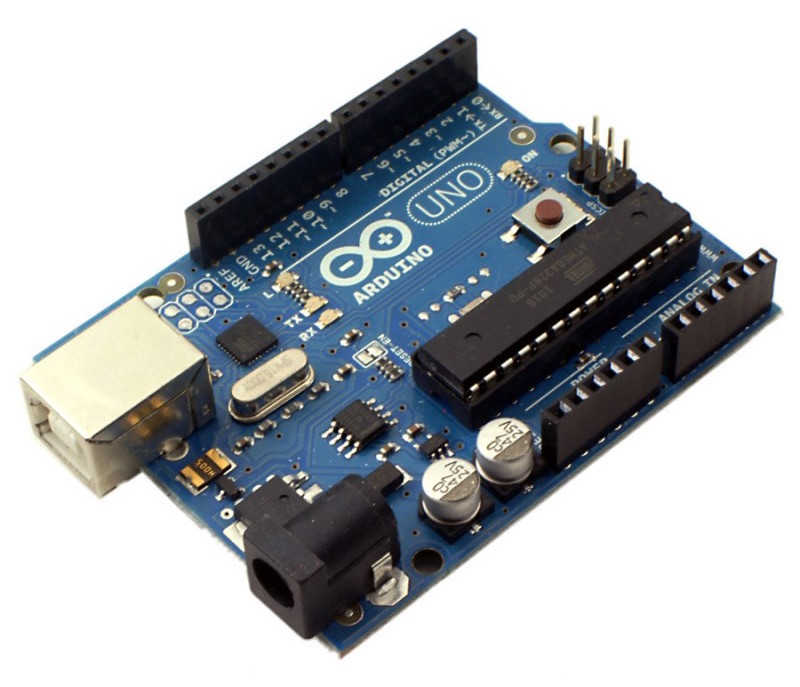
\includegraphics[width=\textwidth]{Files/arduino}
            \caption{An Arduino UNO.}
            \label{fig: arduino}
        \end{subfigure}
        ~
        \begin{subfigure}[b]{0.45\textwidth}
            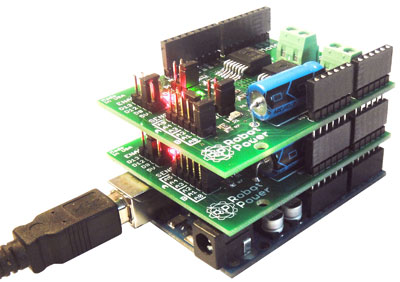
\includegraphics[width=\textwidth]{Files/arduino_with_shields}
            \caption{An Arduino with 2 \glspl{shield} attached.}
            \label{fig: arduino shields}
        \end{subfigure}
        \caption{\small (Retrieved from \citen{robotshop} on 2016--01--25)}
        \label{fig: arduino and shields}
        % \vspace{-20pt}
    \end{figure}
    The robot will need a control system to plan and control its movement, and to control the drawing tool. This system could be developed from proprietary systems or built by the group for this specific application.

    \paragraph{Arduino} (Figure~\ref{fig: arduino}) is an open-source micro-controller system designed for embedded systems control. It can be expanded by the use of \emph{\glspl{shield}} (Figure~\ref{fig: arduino shields}), circuit boards designed to attach to header pins on the primary micro-controller board to created stacks of circuits with different functions. This would allow us to build a control system for the robot using pre-designed circuits. \Glspl{shield}, which can be sourced from many electronics suppliers, are available to add bluetooth, GPS, motor control, and many other functions to the primary circuit.\\
    There is a large online community supporting the Arduino project, which could be leveraged to solve programming difficulties if they arise. The Arduino project provides an integrated development environment (IDE); the Arduino is programmed using a language based on the C and C++ languages.
    \paragraph{Netduino} is a variant of the Arduino which runs on Microsoft's .NET framework. The online support community for this system is smaller, although some group members (\AG, \LY) have a pre-existing familiarity with the .NET framework.\\

\todo[inline]{Electronics: rework the following paragraphs}
    \paragraph{Paspberry Pi}is a small single-board computer developed in the UK to promote access to computer science education in schools. Because on this, the platform is already widely used in an educational setting and thus would allow this project to be more easily integrated into the teaching of computer science. The computer itself is low-cost (<\pounds{50}\todo{check the price of Raspberry Pi}).\\
    The Raspberry Pi Foundation also produce smaller versions of the Raspberry Pi computer which are designed for use in embedded systems. These boards are less customizable than the Arduino system. However, it is compatible with the Python language, which has an extensive support community online and is familiar to all the group, as well as C, C++, Java, and others.

    \paragraph{A micro-controller} integrated circuit could be used in a purpouse-built circuit to control the robot. This would require the design of all the supporting electronics. The microprocessor would need to be programmed in a low-level assembly language or a language designed specifically for the micro-controller product we use.\\
    These components would be cheaper than commercially available systems, but would require much more electronics design work and fabrication.

\section{Summary and decisions}
\towrite{summary and decisions}
    \myBlindSubsection{Aims and motivations}{writer TBA}

    \myBlindSubsection{Drawing tool}{writer TBA}

    \myBlindSubsection{Electronics platform and guidance system}{writer TBA}
    \mySubsection{Outline specification}{\textsc{Whole Group}}\label{outline specification}
        \begin{enumerate} %Reference items in this list using \refspec{drawing size} etc.
            \subsubsection{The project}
            \item We shall design and build a prototype robot to draw 2d line drawings in sand.\label{spec: draw}
            \item The robot shall take input from a user which it shall translate into instructions to draw the picture;\label{spec: take input}
            \item the drawings should be ??? \todo{how big will the drawings be?} in size; \label{spec: drawing size}
            \item the robot should be for educational uses. \label{spec: education}

            \subsubsection{Control systems}
            \item The robot shall be controlled with an Arduino; \label{spec: arduino}
            \item the robot shall use \gls{GPS} for guidance; \label{spec: gps}
            \item the robot should detect objects in front of it. The robot should not collide with objects; \label{spec: detect objects}
            \item the robot should circumvent obstacles.\label{spec: circumvent}

            \subsubsection{The robot hardware}
            \item The robot shall move across the sand using ???\todo{how will it move?}; \label{spec: movement}
            \item the robot shall use ??? \todo{how will it draw?} to draw the images; \label{spec: tool}
            \item the robot shall be built from ??? \todo{what will it be built from?}; \label{spec: material}
            \item the robot shall have dimensions equal to or less than ($56 \times 45 \times 25$) cm. \label{spec: robot size}

            \subsubsection{Safety}
            \item The robot shall have an emergency shut-down switch; \label{spec: kill switch}
            \item the robot should indicate operating faults to the user; \label{spec: error indicator}
            \item the robot should have documentation and instructions for end users. \label{spec: documentation}
            \item The robot should comply with Directive 2009/48/EC of the European Parliament and of the Council of 18 June 2009 on the safety of toys.\cite{EuropeanParliament2009} \label{spec: EU regulations}
        \end{enumerate}
